% !TeX spellcheck = en_US

% GIS Grundlagen
% GIS Libs & Software
% Datenbanken
% MARS Architektur + Rahmenbedingungen
\chapter{Basics}
This chapter elaborates on the fundamental concepts and technologies necessary to understand the following chapters. They consist of a general overview of Geographic Information Systems, the mentioned geospatial libraries and databases, as well as the MARS Eco-System and it's circumstances



\section{Geographic Information System (GIS)}
GIS consists of numerous technologies to store, manipulate, analyze and visualize geographical data. It can be used in all domains that require the use of temporal and spatial data. Some usages are the visualization of land-use, elevation data, weather maps, street networks and flood maps. To leverage the capabilities that GIS offers, specialized software is required that can handle the spatial references, such as ESRI ArcMap QGIS or GrassGIS.


\subsection{Coordinate Reference System (CRS)}
In comparison to normal image data, such as JPEG or PNG, GIS data is geo-referenced, meaning each feature or pixel has a geospatial location. This is achieved by specific geo-aware formats that encode spatial positions into the data. This location is represented in a coordinate system. In GIS terminology this is referred to as \enquote{spatial reference system} (SRS) or \enquote{coordinate reference system} (CRS). Depending on the spatial area, coordinate systems provide different accuracy in their results. Some are optimized for certain areas, while others offer a general worldwide accuracy. The following sections explain common reference systems.

\subsubsection{Mercator Projection}
The most globally used CRS is the Mercator projection. I was created by Gerardus Mercator in 1569 \cite{meer2012atlas} and has been improved over the years. Figure \ref{fig:mercator} shows the Mercator projection in it's normal (left) and transverse (right) orientation. The normal projection offers good general representation, while the transverse orientation is focuses on the poles.
\begin{figure}[H]
	\centering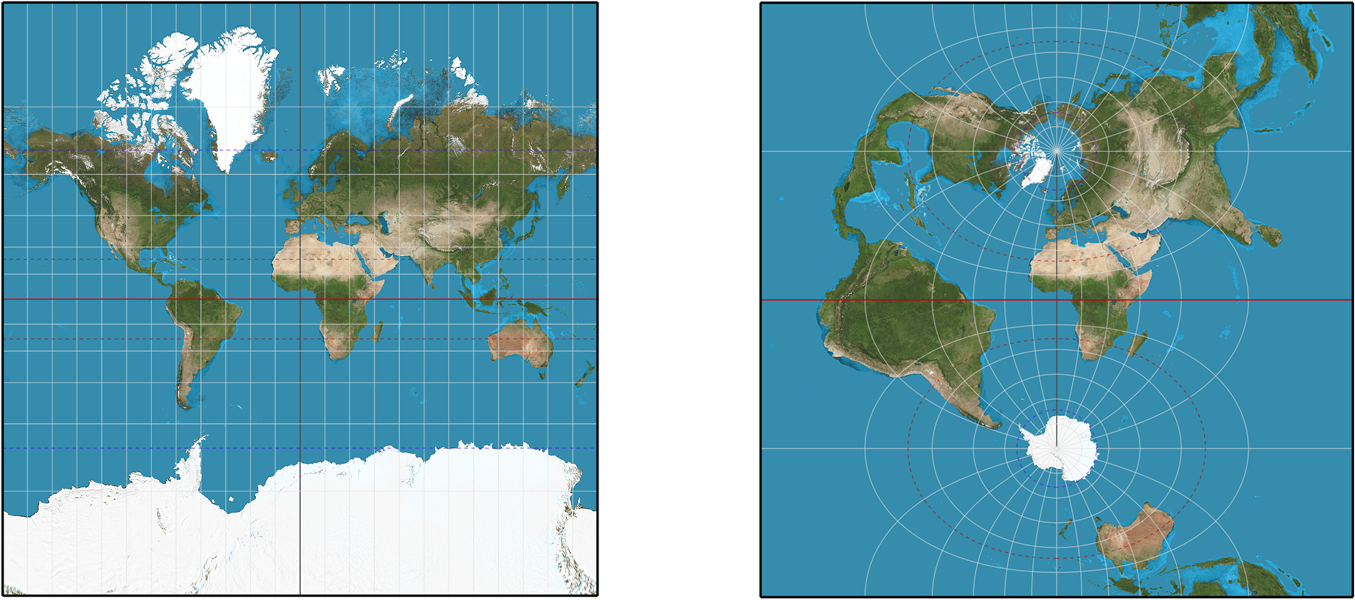
\includegraphics[width=1\textwidth]{res/Mercator}
	\caption{Normal and transverse Mercator projection. \url{https://commons.wikimedia.org/w/index.php?curid=9910866}}
	\label{fig:mercator}
\end{figure}

\subsubsection{EPSG:4326 -- WGS 84}
The most recent version of the Mercator projection is called WGS 84. It improves in accuracy compared to WGS 72 and is an \enquote{European Petroleum Survey Group} (EPSG) standard called EPSG:4326, created by \cite{Decker1986}.\\
WGS 84 is an ellipsoidal coordinate system that shows the 3D surface of the earth in 2D. The coordinates are longitude and latitude measured in degree. Longitude has the 0° point in Greenwich, England and increases east to a maximum of 180° and west to a minimum of -180°. Latitude has the 0° point at the equator and increases north to a maximum of 90° and south to a minimum of -90.\\
WGS 84 is used by the Global Positioning System (GPS), GIS specialists, inside the OpenStreetMap (OSM) database, as well as Google Earth.

\subsubsection{EPSG:3857 -- WGS 84 / Pseudo-Mercator}
Pseudo-Mercator is a projected version of WGS 84 into a two-dimensional cartesian coordinate system. It is also referred to as EPSG:3857 and was created by \cite{Grafarend1995}.\\
The CRS is based on a plane, rather than an ellipse. The zero points is identical to WGS 84 but the coordinates are X and Y measured in meters. The Y coordinate is limited to ±85.06° of the WGS 84 bounds. This results in a square projection with a range of ±20,026,376.39m on both axis, but sacrifices the poles to some extend. The square shape allow the creation of tile pyramids, also called \enquote{Mercator Pyramids} to be used for maps in browsers for the web. \\
A pyramid consists of square images in fixed size, e.g. 256x256px. The First level has one image that shows the whole area of the data with minimal detail. On every level below the number of image tiles increases and therefore the level of detail. The number of tiles on a given level is
$$x_n= 4* x_{n-1}$$ 
where \enquote{x} is the number of tiles and \enquote{n} is the current level of detail. Figure \ref{img:mercator-pyramid} shows an example of a Mercator pyramid.
\begin{figure}[H]
	\centering
	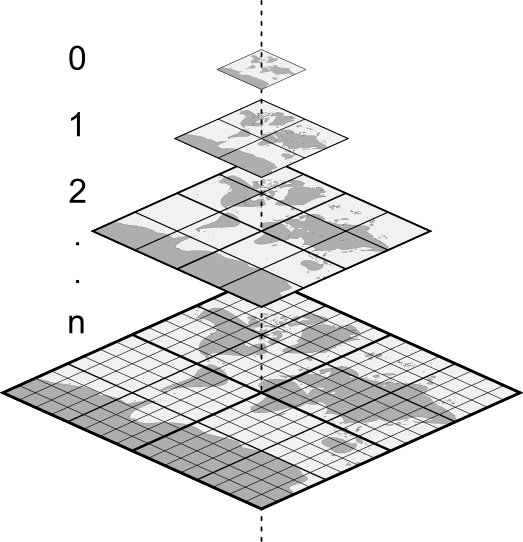
\includegraphics[width=0.4\columnwidth]{res/mercator-pyramid}\\
	\caption[]{Mercator tile pyramid. \url{http://data.webglearth.com/doc/webgl-earthch1.html}}
	\label{img:mercator-pyramid}
\end{figure}
This fragmentation of a big dataset is optimal to be loaded on demand and cached by a web browser, which is why major map sites, like OpenStreetMap, Google Maps and Bing Maps use Pseudo-Mercator as their reference system.


\subsection{Spatial Data Types}
Geo-spatial data exist in two different types, vector and raster. 

\subsubsection{Raster Data}
 Raster data consists of a grid in fixed size. Depending on the file, each pixel contains a color (e.g. satellite data)  or a grayscale (e.g. elevation maps) value.\\
 The advantage of raster data is that it is better suited to store picture like data with gradients. Due to its nature, raster has data in every cell, which leads into a high amount of data that has to be stored, so the potential file size if big.\\
 Since the raster size is fixed, the balance between desired detail and small file size has to be decided upon file creation. Figure \ref{img:raster} shows a shape in three different rasterized resolutions, visualizing the loss of detail.
 \begin{figure}[H]
 	\centering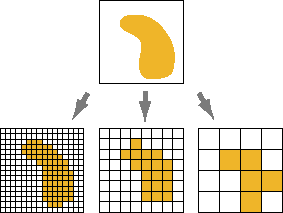
\includegraphics[width=.5\textwidth]{res/Vector-Raster}
 	\caption{Shape as raster in different resolutions. \url{http://desktop.arcgis.com/en/arcmap/latest/manage-data/raster-and-images/what-is-raster-data.htm}}
 	\label{img:raster}
 \end{figure}
Common file types for raster data are GeoTIFF, ESRI, ESRI ArcGrid and ASCIIGrid. GeoTIFF and ArcGrid are binary file types and ASCIIGrid is text-based.

\subsubsection{Vector Data}
In contrary to raster data, vectors files don't map color information to a specific pixel, but define mathematical shapes which are rendered as desired. This allows very efficient storage and it is possible to scale the shapes as desired.\\
Data inside vector GIS can have several layers. Each layer can be of the type points, line or polygon. The data on a layer is called a feature. A point feature has a single coordinate, like a well. lines are open polygon lines and are often used for rivers. Shapes are closed lines and are used for areas like countries, lakes, or larger objects. Figure \ref{img:vector} shows a vector file with 3 layers. The point layer shows the position of wells, the linestring layer shows a river and the polygon layer a lake.\\
\begin{figure}[H] 
	\centering
	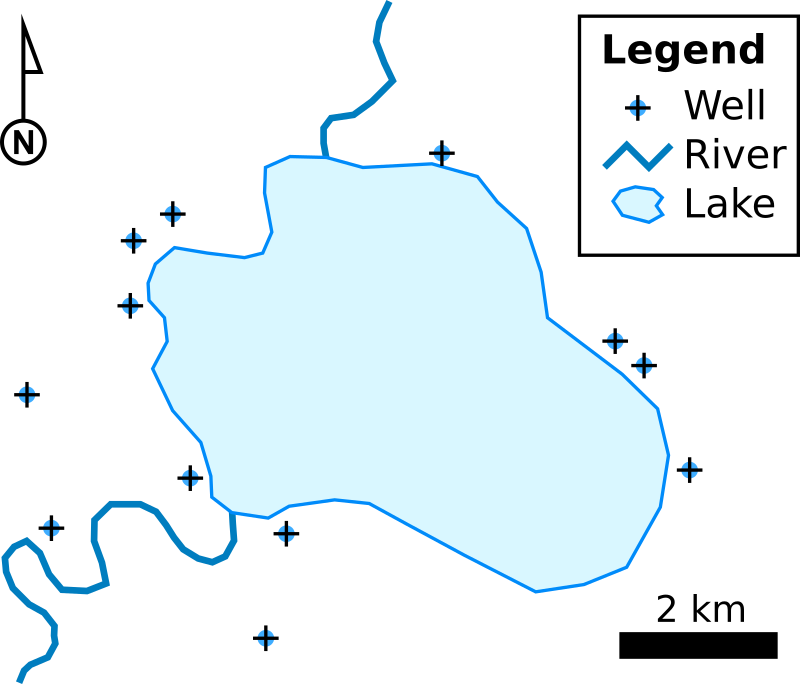
\includegraphics[width=0.4\columnwidth]{res/vector-map}\\
	\caption[]{Vector map with point, line and polygon. \url{https://commons.wikimedia.org/w/index.php?curid=3024482}}
	\label{img:vector}
\end{figure}

Vector GIS is however limited in its capabilities. The mathematical functions mentioned above are not well suited for data without discrete values. Anything that has gradients is better suited for raster.\\
The most common vector file formats are ESRI Shapefile as binary and GeoJSON as a text-based format.



\section{GIS Technologies}
Chapter \ref{sec:software_design} and \ref{sec:implementation} discuss technologies that were considered at one point of this work. The following section introduces them briefly.


% Performance tests hier???
\subsection{Spatial Databases}
Spatial databases are DBs that have been extended to store and query spatial data types.

\subsubsection{PostGIS}
PostGIS \citep{Obe2011} is an extended PostgreSQL that allows to store and query both raster and vector GIS.

\subsection{Spatial Libraries}



\section{MARS}
MARS (Multi-Agent Research and Simulation) is a working group at the HAW (University of applied Sciences) in Hamburg, Germany. The research group develops an distributed agent-based simulation system to be used by domain experts around the world. It consists of several components.


\subsection{LIFE}
The simulation system is called MARS LIFE. It executes simulation runs created inside the Cloud Services. For more detail see \cite{Huning2016}.


%\subsection{Cloud Services}
%The Cloud Services are the central back-end of the MARS system. These components are responsible for data import, persistence, data visualization an the connection between LIFE and the WebUI.
%
%
%\subsection{WebUI}
%The WebUI is the front-end of MARS. It is a web-based application that allows the user to control back-end services and trigger simulations from the web-browser.


%\section{Mono}
%Open C\# implementation for Linux and OSX.
%
%
%
%\section{.NET Core}
%Microsoft bought Xamarin, which mostly developed Mono and is creating it's new C\# with build in multi-platform support.